\documentclass[10pt,a4paper]{article}
\usepackage[utf8]{inputenc}
\usepackage{graphicx}
\usepackage[left=1.0in, right=1.0in, top=1.0in, bottom=1.0in]{geometry}
\usepackage[swedish]{babel}
\usepackage{tikz}
\usetikzlibrary{arrows.meta,shapes,calc,backgrounds}
\usepackage{parskip}
\usepackage{xcolor}
\usepackage[most]{tcolorbox}
\usepackage{mdframed}
\usepackage{tabularx}
\usepackage{colortbl}
\usepackage{enumerate}
\usepackage{enumitem}

\setlength{\extrarowheight}{8pt}
\renewcommand{\arraystretch}{1}

% My colors
\definecolor{mycolor1}{rgb}{1,0,0} %red
\definecolor{lightpurple}{HTML}{c69cd6}
\definecolor{darkpurple}{HTML}{7b5c87}

%circled
\newcommand*\circled[1]{\tikz[baseline=(char.base)]{
		\node[shape=circle,draw,minimum size=1em, inner sep=2pt] (char)
		{#1};}
}

% Purpleleftline
\newmdenv[innerleftmargin=20,topline=false,rightline=false,bottomline=false, linewidth=3pt, linecolor=darkpurple]{purpleleftline}

% Kommentarboxen
\tikzstyle{mybox} = [draw=lightpurple!35, fill=lightpurple!35, very thick,
rectangle, inner sep=15pt, inner ysep=15pt]
\tikzstyle{fancytitle} =[fill=darkpurple, text=white]

% Title format
\newcommand{\pagetitle}[2] {
	\begin{tabularx}{\linewidth}{>{\columncolor{darkpurple}}c >{\columncolor{lightpurple!35}}X}
		\LARGE \textcolor{white}{{#1}} & \LARGE {#2} \\[3pt]
	\end{tabularx}
}

% Instruction environment
\newenvironment{instructionsenv}
{
	\vspace{-4pt}
	\begin{purpleleftline}
		\vspace{2em}
		{\Large\bfseries{Instruktioner}}\par
		\vspace{1em}
	}
	{ 
	\end{purpleleftline}
}

% Instruction
\newcommand{\instruction}[2] {
	\textcolor{mycolor1}{\circled{\large {#1}}} 
	{\large #2}\par
}

% Kommentarbox
\newcommand{\kommentarbox}[1]{
	\begin{center}
		\begin{tikzpicture}
		\node [mybox] (box){%
			\begin{minipage}{0.91\textwidth}
			{#1}
			\end{minipage}
		};
		\node[fancytitle, right=15pt] at (box.north west) {\bfseries Kommentar};
		\end{tikzpicture}
	\end{center}	
}

\begin{document}

%%%%%%%%%%%%%%%%%%%%%%%%%%%%%%%%%%%%%%%%%%%%%%%%%%%%%%%%%%%%%%
%%% Titelsidan
%%%%%%%%%%%%%%%%%%%%%%%%%%%%%%%%%%%%%%%%%%%%%%%%%%%%%%%%%%%%%%
\pagenumbering{gobble}
\newgeometry{left=0cm,bottom=0cm,right=0cm,top=0cm}

\begin{tikzpicture}

\fill[lightpurple!35] (0,0) rectangle (\paperwidth,\paperheight);

\fill[white] (0,0) rectangle (0.65\paperwidth,\paperheight);

\fill[darkpurple] (0,0.45\paperheight) rectangle (\paperwidth,0.65\paperheight);

\node[align=left,white] at (0.5\paperwidth,0.57\paperheight) 
{\bfseries\Huge Exempel på användande av \\ \bfseries\Huge EMG-utrustningen på HSC};

\node[align=center,white] at (0.5\paperwidth,0.505\paperheight) 
{ \huge En praktisk guide};

\node[align=center,black] at (0.825\paperwidth,0.1\paperheight) 
{\Large Peter Kvillegård \\[3em] Version 1.0 \\ 2020-01-23};

\end{tikzpicture}
\restoregeometry
\newpage

%%%%%%%%%%%%%%%%%%%%%%%%%%%%%%%%%%%%%%%%%%%%%%%%%%%%%%%%%%%%%%
%%% Bakgrund
%%%%%%%%%%%%%%%%%%%%%%%%%%%%%%%%%%%%%%%%%%%%%%%%%%%%%%%%%%%%%%

\pagetitle{Om denna guide}{}\par
\vspace{1em}
Jag och Jonatan Malmström använde under hösten 2019 EMG-utrustningen på HSC i Lund för ett experiment. Vi lärde oss att använda program och apparater av andra elever och av vår handledare. I denna användarguide har vi skrivit ner hur vi använde utrustningen, i förhoppning om att det kan vara användbart för andra.

Utrustningen som användes och beskrivs här är MegaWin 3.01b mjukvara med ???? hårdvara.  

Vårt arbete fokuserade på att få fram medelamplitud under en definierad tid i olika muskler samtidigt, och användarguiden är därför inriktad för det ändamålet. Detta är inte är en allomfattande manual, utan ett exempel på hur utrustningen kan användas. Det är mycket möjligt att det finns bättre och smidigare sätt, och det finns många andra ändamål som inte kommer att beskrivas här.

All text och bilder är tillgängliga under Creative Commons 0 (CC0), vilket i princip innebär att vem som helst har rätt att göra vad som helst med innehållet.
Källkoden är skriven i \LaTeX{} och finns att hitta tillsammans med bilderna på \verb|http://www.github.com/mouboo/lund_emg_userguide|. Om du upptäcker fel eller vill bygga vidare på denna guide är du mycket välkommen att göra så, kontakta mig på \verb|peterkvillegård@gmail.com| för mer information om detta.

\newpage

%%%%%%%%%%%%%%%%%%%%%%%%%%%%%%%%%%%%%%%%%%%%%%%%%%%%%%%%%%%%%%
%%% Innehåll
%%%%%%%%%%%%%%%%%%%%%%%%%%%%%%%%%%%%%%%%%%%%%%%%%%%%%%%%%%%%%%

\pagetitle{Innehåll}{}\par
\vspace{3em}
{\Large

\begin{enumerate}[label={\Roman*},align=left]
\item Logga in \dotfill 1
\item Skapa protokoll \dotfill 2
\item Skapa person \dotfill 3
\item Anslut biomonitor \dotfill 4
\item Kontrollera signalen \dotfill 5
\item Utför mätning \dotfill 6
\item Bearbeta signalen \dotfill 7
\end{enumerate}
}

\newpage
\pagenumbering{arabic}

%%%%%%%%%%%%%%%%%%%%%%%%%%%%%%%%%%%%%%%%%%%%%%%%%%%%%%%%%%%%%%
%%% Logga in | Steg 1/1
%%%%%%%%%%%%%%%%%%%%%%%%%%%%%%%%%%%%%%%%%%%%%%%%%%%%%%%%%%%%%%

%%%%% Title
\pagetitle{I. Logga in}{Steg 1/1}

%%%%% Instruktioner
\begin{instructionsenv}
	\instruction{1}{Kryssa i ``Workstation only''}
	\instruction{2}{Fyll i Username: \texttt{emg}, Password: \texttt{emgemg}}
	\instruction{3}{Klicka på ``OK''}
\end{instructionsenv}

\vspace{50pt}

%%%%% Bilden
\begin{center}
	\begin{tikzpicture}
	\node[anchor=south west,inner sep=0] (image) at (0,0) {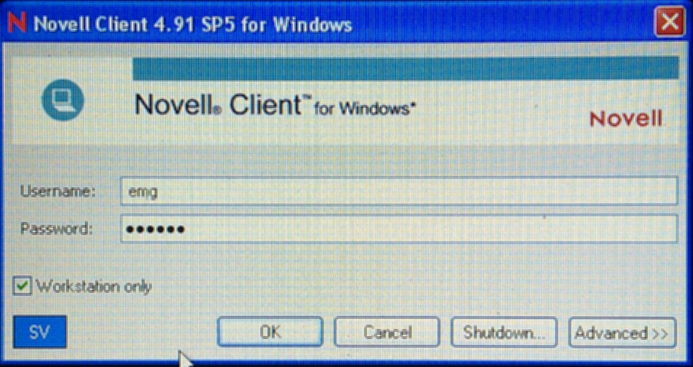
\includegraphics[width=0.5\textwidth]{./img/login}};
	\begin{scope}[x={(image.south east)},y={(image.north west)}]
	
	%Cirkel med streck och referens 1
	\node[mycolor1, thick] (A) at  (0.2,0.1) {\Large 1};
	\node[circle, draw, mycolor1, thick, minimum size=0.5cm] (B) at  (0.03,0.22) {};
	\draw[mycolor1, thick] (A) -- (B);

	%Cirkel med streck och referens 2
	\node[mycolor1, thick] (A) at  (0.5,0.6) {\Large 2};
	\node[circle, draw, mycolor1, thick, minimum size=1.2cm] (B) at  (0.22,0.43) {};
	\draw[mycolor1, thick] (A) -- (B);
	
	%Cirkel med streck och referens 3
	\node[mycolor1, thick] (A) at  (0.6,0.25) {\Large 3};
	\node[circle, draw, mycolor1, thick, minimum size=0.8cm] (B) at  (0.39,0.1) {};
	\draw[mycolor1, thick] (A) -- (B);

	\end{scope}
\end{tikzpicture}
\end{center}

\vspace{35pt}

\newpage

%%%%%%%%%%%%%%%%%%%%%%%%%%%%%%%%%%%%%%%%%%%%%%%%%%%%%%%%%%%%%%
%%% II. Skapa protokoll | Steg 1/?
%%%%%%%%%%%%%%%%%%%%%%%%%%%%%%%%%%%%%%%%%%%%%%%%%%%%%%%%%%%%%%

%%%%% Title
\pagetitle{II. Skapa protokoll}{Steg 1/?}

%%%%% Instruktioner
\begin{instructionsenv}
	\instruction{1}{Klicka på ``Protocol''}
\end{instructionsenv}

\vspace{50pt}

%%%%% Bilden
\begin{center}
\begin{tikzpicture}
	\node[anchor=south west,inner sep=0] (image) at (0,0) {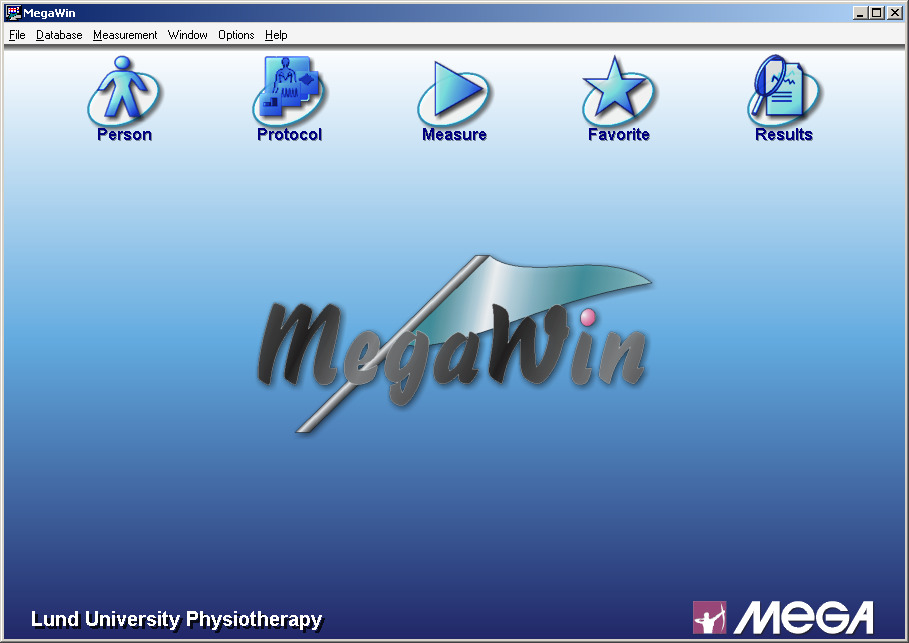
\includegraphics[width=0.91\textwidth]{./img/3}};
	\begin{scope}[x={(image.south east)},y={(image.north west)}]
		
	%Cirkel med streck och referens
	\node[mycolor1, thick] (A) at  (0.2,0.6) {\Large 1};
	\node[circle, draw, mycolor1, thick, minimum size=2cm] (B) at  (0.32,0.85) {};
	\draw[mycolor1, thick] (A) -- (B);

	\end{scope}
\end{tikzpicture}
\end{center}

\vspace{35pt}

%%%%% Kommentarboxen
\kommentarbox{
	Paragraf som förklarar vad som händer i detta stycke. Det är möjligtvis lite längre, för att få kontext vad som händer, och för att kunna förstå vad man gör. Detta möjliggör att man kan ta egna vägar senare och experimentera med funktionaliteten i programmet.
}
\newpage

%%%%%%%%%%%%%%%%%%%%%%%%%%%%%%%%%%%%%%%%%%%%%%%%%%%%%%%%%%%%%%
%%% II. Skapa protokoll | Steg 2/?
%%%%%%%%%%%%%%%%%%%%%%%%%%%%%%%%%%%%%%%%%%%%%%%%%%%%%%%%%%%%%%

%%%%% Title
\pagetitle{II. Skapa protokoll}{Steg 2/?}

%%%%% Instruktioner
\begin{instructionsenv}
	\instruction{1}{Klicka på ``New...''}
\end{instructionsenv}

\vspace{50pt}

%%%%% Bilden
\begin{center}
	\begin{tikzpicture}
	\node[anchor=south west,inner sep=0] (image) at (0,0) {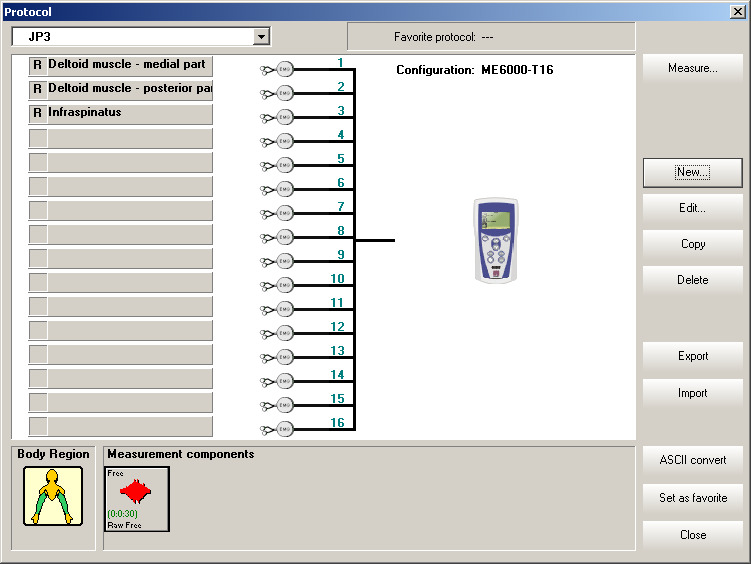
\includegraphics[width=0.8\textwidth]{./img/7}};
	\begin{scope}[x={(image.south east)},y={(image.north west)}]
	
	%Cirkel med streck och referens
	\node[mycolor1, thick] (A) at  (0.75,0.75) {\Large 1};
	\node[circle, draw, mycolor1, thick, minimum size=1cm] (B) 
	at  (0.92,0.7) {};
	\draw[mycolor1, thick] (A) -- (B);
	
	\end{scope}
	\end{tikzpicture}
\end{center}

\vspace{35pt}
\newpage

%%%%%%%%%%%%%%%%%%%%%%%%%%%%%%%%%%%%%%%%%%%%%%%%%%%%%%%%%%%%%%
%%% II. Skapa protokoll | Steg 2/?
%%%%%%%%%%%%%%%%%%%%%%%%%%%%%%%%%%%%%%%%%%%%%%%%%%%%%%%%%%%%%%

%%%%% Title
\pagetitle{II. Skapa protokoll}{Steg 3/?}

%%%%% Instruktioner
\begin{instructionsenv}
	\instruction{1}{Fyll i protokollets namn}
	\instruction{1}{Välj ``Advanced protocol''}
	\instruction{1}{Klicka på ``Next''}
\end{instructionsenv}

\vspace{50pt}

%%%%% Bilden
\begin{center}
	\begin{tikzpicture}
	\node[anchor=south west,inner sep=0] (image) at (0,0) {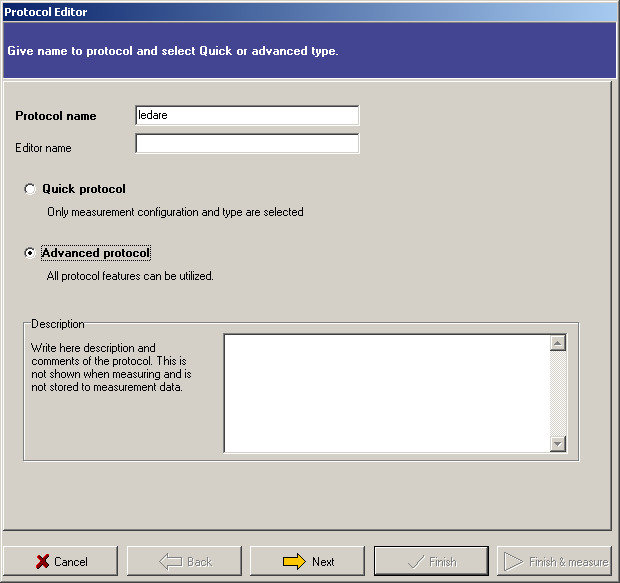
\includegraphics[width=0.8\textwidth]{./img/8}};
	\begin{scope}[x={(image.south east)},y={(image.north west)}]
	
	%Cirkel med streck och referens 1
	\node[mycolor1, thick] (A) at  (0.55,0.7) {\Large 1};
	\node[circle, draw, mycolor1, thick, minimum size=1cm] (B) 
	at  (0.25,0.8) {};
	\draw[mycolor1, thick] (A) -- (B);
	
	%Ellips med streck och referens 2
	\node[mycolor1, thick] (A) at  (0.5,0.55) {\LARGE 2};
	\node[ellipse, draw, mycolor1,thick,minimum height=0.9cm,minimum width=3.5cm,draw] (B) at  (0.15,0.565) {};
	\draw[mycolor1, thick] (A) -- (B);
	
	%Ellips med streck och referens 2
	\node[mycolor1, thick] (A) at  (0.5,0.3) {\LARGE 3};
	\node[ellipse, draw, mycolor1,thick,minimum height=0.7cm,minimum width=2.5cm,draw] (B) at  (0.495,0.037) {};
	\draw[mycolor1, thick] (A) -- (B);
		
	\end{scope}
	\end{tikzpicture}
\end{center}

\vspace{35pt}
%%%%% Kommentarboxen
\kommentarbox{
	I denna guide har jag valt att kalla protokollet ``ledare'', döp gärna ert protokoll till något unikt som ni kommer ihåg, exempelvis försöksledarnas initialer.
}
\newpage

\end{document}